% Governance-Gated Credit-Risk Benchmarking
% Technical report for github.com/asynced24/bayesian-credit-risk-gate
%
% Build:
%   python main.py --sample
%   python main.py                                    (full 30,000 rows, Section 5.5)
%   python docs/figures/generate_figures.py
%   pdflatex -interaction=nonstopmode whitepaper.tex   (run twice, from docs/)
%
% Every figure and every number in this document comes from one of those two runs -
% the sample run of Section 4 unless the text says otherwise. Nothing is illustrative.

\documentclass[10pt,a4paper]{article}

\usepackage{lmodern}
\usepackage[T1]{fontenc}
\usepackage[utf8]{inputenc}
\usepackage[margin=0.9in]{geometry}
\usepackage{graphicx}
\usepackage{amsmath}
\usepackage{amssymb}
\usepackage{booktabs}
\usepackage{caption}
\usepackage{microtype}
\usepackage[hidelinks]{hyperref}

\graphicspath{{figures/}}

\captionsetup{font=small,labelfont=bf,width=0.95\textwidth,skip=5pt}
\setlength{\parskip}{0.2em}

% Tighter section spacing than the article defaults, to keep the report compact.
\makeatletter
\renewcommand\section{\@startsection{section}{1}{\z@}%
  {-2.2ex \@plus -0.6ex \@minus -.2ex}{1.0ex \@plus .2ex}%
  {\normalfont\large\bfseries}}
\renewcommand\subsection{\@startsection{subsection}{2}{\z@}%
  {-1.8ex \@plus -0.5ex \@minus -.2ex}{0.7ex \@plus .2ex}%
  {\normalfont\normalsize\bfseries}}
\makeatother

% Let floats share pages with text rather than taking pages of their own.
\renewcommand{\topfraction}{0.92}
\renewcommand{\bottomfraction}{0.85}
\renewcommand{\textfraction}{0.07}
\renewcommand{\floatpagefraction}{0.80}
\setlength{\textfloatsep}{12pt plus 3pt minus 3pt}
\setlength{\intextsep}{12pt plus 3pt minus 3pt}

\newcommand{\code}[1]{\texttt{\small #1}}

\title{\vspace{-1.2cm}\textbf{Governance-Gated Credit-Risk Benchmarking:\\
Empirical-Bayes Segment Shrinkage on the UCI\\
Default of Credit Card Clients Dataset}}

\author{Aryan Singh\\
\small\href{https://github.com/asynced24/bayesian-credit-risk-gate}%
{github.com/asynced24/bayesian-credit-risk-gate}\ \ (\code{v1.0.0})}

\date{August 2026}

\begin{document}

\maketitle

\begin{abstract}
\noindent
Model selection and model approval ask different questions of a credit-risk
model, and they are usually answered by different artefacts at different times.
This report describes a pipeline that answers both in one run. Three
credit-default models are benchmarked on the UCI \emph{Default of Credit Card
Clients} dataset and each is then put through five governance gates --- fairness,
drift, calibration, uncertainty, and a Bayesian segment-stability check --- whose
thresholds are declared in configuration and validated at startup. Segment-level
default rates, the unit most governance questions are posed in, are estimated
with an empirical-Bayes Beta-Binomial model rather than taken raw, so that cells
holding a handful of borrowers get a defensible rate and an honest interval
instead of noise. On the committed offline sample all three models fail the
combined verdict. The binding finding is an equalized-odds gap of $0.1617$ on
\code{sex} for logistic regression, against a fail limit of $0.10$ --- produced by
a model that never received \code{sex} as a feature. Its $95\%$ interval is
$[0.050, 0.274]$, so the point estimate clears the limit by about one standard
error, and on the full $30{,}000$-row dataset the same gap falls to $0.0245$ while
the fairness gate still fails, on \code{age\_band}: the mechanism reproduces, the
magnitude does not. A second finding is that governance verdicts reproduce across
platforms while the benchmark ranking does not: XGBoost's histogram tree builder
moves ROC-AUC by more than the margin separating the top two models.
\end{abstract}

\section{Problem statement}

A credit-scoring model has to pass model-risk review before it can inform a
lending decision, and review asks a different set of questions from the ones
model selection asks. Selection asks which model ranks borrowers best. Review
asks whether a predicted probability means what it claims, whether error rates
are comparable across demographic groups, whether the input distribution has
moved since training, and whether an individual adverse decision can be
explained to the person who received it.

Those two sets of questions are normally answered by separate artefacts: a
training script produces the discrimination metrics, and a document assembled
weeks later addresses the review questions, often from summary statistics rather
than from a check that runs. The separation matters because the two can
disagree, and a model with the best ROC-AUC in a benchmark can still be one that
should not be deployed.

This framework runs both in the same pipeline. Every threshold lives in
\code{config.yaml}, is validated by pydantic at startup, and yields a
pass/warn/fail verdict on every run; the worst gate becomes the model's verdict.
Selection and approval are separate outputs of a single execution.

A second concern is segment granularity. Governance questions are usually posed
per demographic segment, and a segment default rate computed directly is
dominated by sampling noise once the cell is small: in the run reported here, one
segment holds six borrowers and zero defaults, and its raw default rate of
$0.000$ is not a usable input to any provisioning decision. Section~\ref{sec:eb}
describes the empirical-Bayes model used in place of raw rates.

\section{Architecture}

Figure~\ref{fig:arch} shows the pipeline. The loader fetches UCI dataset 350,
caches it, and can instead read a committed 5{,}000-row class-stratified sample
so that the whole pipeline runs with no network access. The processor engineers
28 behavioural features from the six months of billing and repayment history,
giving 49 predictors, and splits the data. It also separates \emph{audit
columns} from the feature matrix: \code{sex} and \code{marriage} are withheld
from training entirely as prohibited bases and retained only so the fairness
gate can measure against them.

Two components then feed the gates. The benchmark suite fits the three models
and produces test-set predictions and metrics. Independently, the shrinkage
model fits a population prior and per-segment posteriors on the training split.
The five gates consume both, and each returns a pass/warn/fail verdict with the
metric and threshold that produced it. Explainability and reporting run after
the gates, and every parameter and metric is logged to MLflow or, when MLflow is
disabled, to a local JSON run log.

\begin{figure}[htbp]
\centering
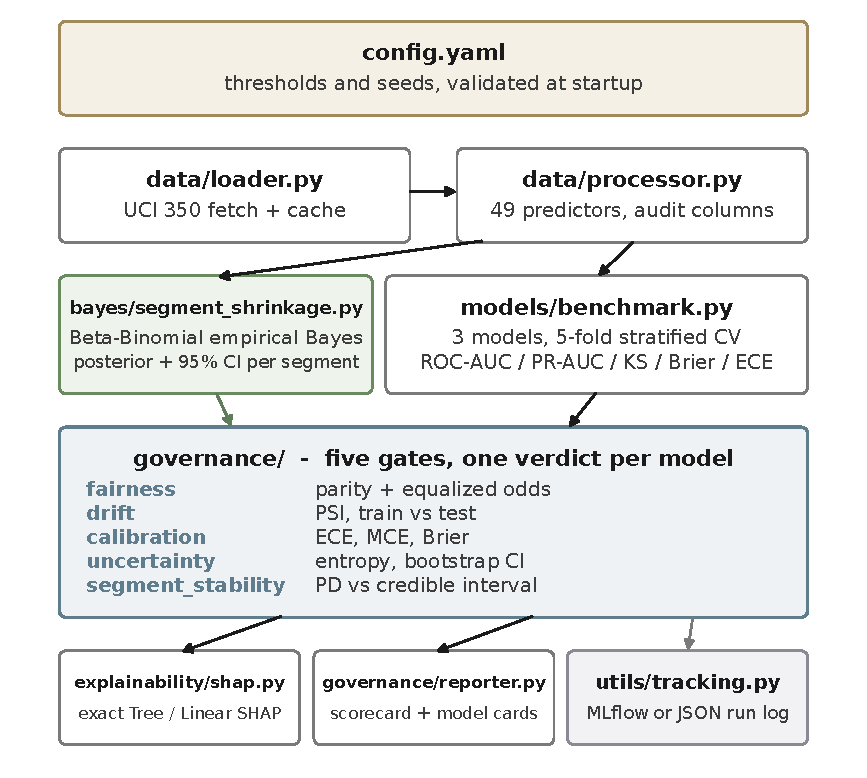
\includegraphics[width=0.67\textwidth]{fig_architecture.pdf}
\caption{Pipeline stages. Thresholds, seeds and the model list are declared once
in \code{config.yaml} and read by every stage below it. The benchmark suite and
the empirical-Bayes shrinkage model are independent inputs to the gate layer:
the first supplies predicted probabilities, the second the segment posteriors
the stability gate compares them against.}
\label{fig:arch}
\end{figure}

\section{Empirical-Bayes segment shrinkage}
\label{sec:eb}

Segments are defined as the cross of education level and age band. Education has
four levels once the codes the source paper leaves undocumented are folded into
its ``other'' category, and age is binned on the edges $20, 30, 40, 50, 60, 80$
declared in \code{config.yaml}, left-closed and right-open, giving the five bands
20--30 through 60--80. The cross is chosen because education and age are the two
demographic columns the model is actually allowed to use as predictors:
\code{sex} and \code{marriage} are withheld as prohibited bases, so segmenting on
them would define the governance unit in terms of a column no lending decision may
depend on, and segmenting on a behavioural feature would make the reference cell a
function of the same history the model is scoring. Four levels times five bands is
20 possible cells, of which 19 appear here --- \code{other\_unknown | 60-80} holds
four borrowers in the full 30{,}000-row dataset and none of them are drawn into the
committed 5{,}000-row sample, so the cell is absent rather than dropped.

Rather than take each cell's observed default rate, the
framework treats the counts hierarchically: each segment has its own latent
default rate, and those rates are themselves draws from one population-level
distribution. Because the Beta is conjugate to the Binomial, every segment's
posterior is closed form, and its mean is automatically a precision-weighted
blend of the segment's own rate and the population rate. The weight is not a
tuned constant --- it falls out of the posterior algebra, so a thin cell shrinks
hard toward the population rate and a well-populated cell barely moves. For
segment $i$ with $n_i$ borrowers and $k_i$ defaults:
%
\begin{align}
\theta_i &\sim \mathrm{Beta}(\alpha, \beta), &
k_i &\sim \mathrm{Binomial}(n_i, \theta_i), \\[0.3em]
\theta_i \mid k_i, n_i &\sim \mathrm{Beta}(\alpha + k_i,\ \beta + n_i - k_i), \\[0.3em]
\mathbb{E}[\theta_i \mid k_i, n_i]
  &= w_i \frac{k_i}{n_i} + (1 - w_i)\frac{\alpha}{\alpha + \beta},
& w_i &= \frac{n_i}{n_i + \alpha + \beta}.
\label{eq:post}
\end{align}
%
The $95\%$ credible interval is read off the same posterior as the $2.5$th and
$97.5$th percentiles of $\mathrm{Beta}(\alpha + k_i,\ \beta + n_i - k_i)$.

The prior $(\alpha, \beta)$ is estimated by method of moments across segments,
with one correction that matters. The observed spread of the empirical rates
$p_i = k_i / n_i$ overstates the spread of the underlying $\theta_i$, because
each $p_i$ carries its own binomial sampling noise:
%
\begin{equation}
\operatorname{Var}(p_i) = \operatorname{Var}(\theta_i)
  + \mathbb{E}\!\left[\frac{\theta_i(1-\theta_i)}{n_i}\right].
\label{eq:varsplit}
\end{equation}
%
Subtracting the sampling component gives
$\operatorname{Var}(\theta_i) = \operatorname{Var}(p_i) - \overline{\mu(1-\mu)/n_i}$,
floored at a small positive constant, and the Beta concentration then follows
from the identity $\operatorname{Var}(\theta_i) = \mu(1-\mu)/(\alpha + \beta + 1)$.
Using $\operatorname{Var}(p_i)$ directly instead yields a prior that is too diffuse
and therefore under-shrinks. Only segments with $n_i \ge 30$ contribute to the prior
fit; every segment receives a posterior regardless.

On the run reported here, 12 of the 19 segments cleared the prior-fitting floor.
The pooled rate is $\mu = 0.2230$, the observed variance of segment rates is
$1.4581 \times 10^{-3}$ and the estimated binomial sampling variance is
$1.0243 \times 10^{-3}$, leaving $\operatorname{Var}(\theta_i) = 4.3375 \times
10^{-4}$. That gives a concentration of $\mu(1-\mu)/\operatorname{Var}(\theta_i) -
1 = 398.49$ and a prior of $\mathrm{Beta}(88.87, 309.62)$ --- in other words, a
prior worth about 398 equivalent borrowers.

$\operatorname{Var}(p_i)$ is taken unweighted across those 12 segments, which is
the consistent reading of the model: each segment contributes one draw of
$\theta_i$, so weighting the spread by $n_i$ would estimate the dispersion of
$\theta$ across borrowers rather than across segments, and would let the two or
three largest cells set the prior for all of them. The choice is not free
numerically --- size-weighting the same 12 segments, sampling term included, gives
a concentration of $352.70$ rather than $398.49$, a prior worth about $11\%$ fewer
equivalent borrowers --- but it moves no posterior far enough to change a gate
verdict in this run.

Two limitations of the construction are worth stating rather than leaving to be
noticed. First, $(\alpha, \beta)$ is estimated from 12 segments and then treated as
known when the posteriors and their credible intervals are formed. The intervals
reported here are therefore conditional on $(\hat\alpha, \hat\beta)$ and understate
the true uncertainty by whatever is attributable to having estimated the
hyperparameters from a small number of cells --- the standard critique of empirical
Bayes~\cite{gelman2013}. A fully Bayesian treatment with a hyperprior, or a
parametric bootstrap over the prior fit, would widen them; on 12 segments the
correction would not be negligible. Second, the model assumes the segment rates are
exchangeable draws from one population distribution. That is an assumption about
education $\times$ age-band cells, not a property of them that this run tests, and
no covariate structure enters the prior: a 60-something with a graduate degree
borrows the same prior as a 20-something who did not finish high school. A
covariate-adjusted small-area model --- Fay-Herriot, say, letting the prior mean
depend on education and age directly --- is the natural extension, and it would
matter most for exactly the thin cells shrinkage exists to rescue.

Figure~\ref{fig:eb} shows the effect. The seven segments left of the boundary
sit below the prior-fitting floor, and their raw rates scatter from $0.000$ to
$0.333$ while their posteriors all sit within a few points of the population
rate with wide intervals. The thinnest, \code{other\_unknown | 50-60}, has
$n = 6$ and $k = 0$: its posterior is $\mathrm{Beta}(88.87, 315.62)$, mean
$0.220$, interval $[0.181, 0.261]$, and by Equation~\ref{eq:post} the weight on
its own data is $6 / (6 + 398.49) = 0.01$. To the right, posteriors track their
raw rates closely and the intervals tighten. Across all 19 segments the median
interval width is $0.0732$ and the median weight on own data is $0.212$.

\begin{figure}[htbp]
\centering
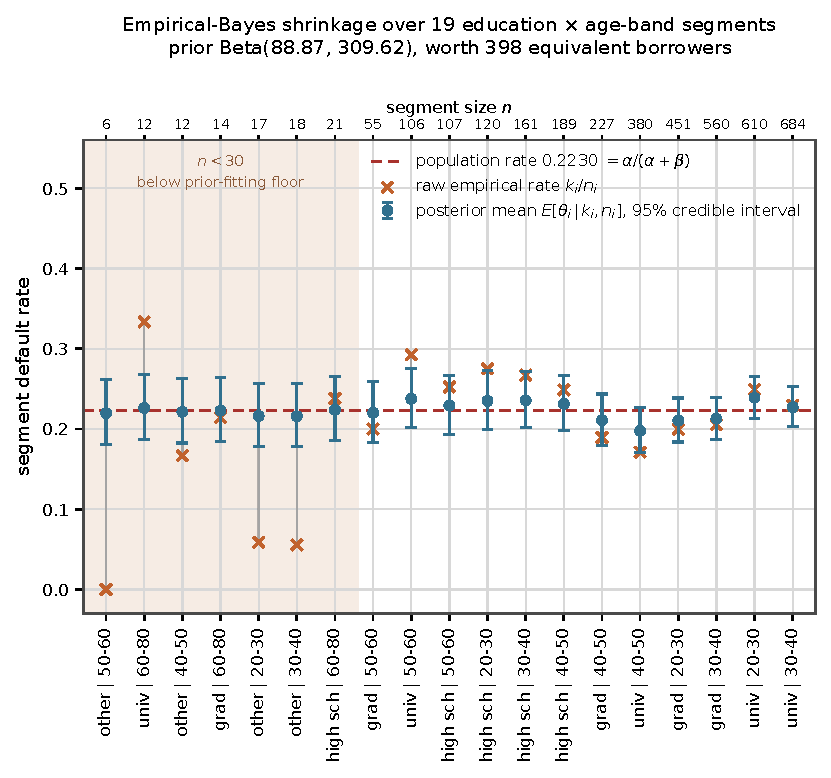
\includegraphics[width=0.72\textwidth]{fig_segment_shrinkage.pdf}
\caption{Raw versus shrunken segment default rates, 19 education $\times$
age-band segments ordered by segment size (sizes on the top axis). Crosses are
the raw empirical rates $k_i/n_i$; circles are posterior means with $95\%$
credible intervals; the grey stems show how far shrinkage moved each estimate.
Thin segments (shaded, $n < 30$) collapse toward the population rate with wide
intervals; well-populated segments barely move. Produced by fitting the model on
the training split of the committed sample.}
\label{fig:eb}
\end{figure}

The segment-stability gate then compares each model's mean predicted probability
of default per segment against these intervals, and flags any segment where the
model prices the cell differently from its noise-corrected historical
experience.

\section{Benchmark results}
\label{sec:bench}

Table~\ref{tab:bench} and Figure~\ref{fig:bench} report a run of
\code{python main.py --sample} at seed 42 on the committed sample (hash
\code{b1ba275532b83033}, base rate $0.2212$), 3{,}750 train and 1{,}250 test
rows, 49 predictors. The split is stratified on the target, so both halves carry
the base rate to three decimal places ($0.221$ train, $0.221$ test) and the
cross-validation folds within the training split are stratified as well.

Class weights are left at their natural values throughout, because rebalancing
buys nothing measurable here and costs the calibration that the ECE and Brier
gates exist to measure. Refitting with \code{class\_weight="balanced"} moves test
ROC-AUC by $+0.0016$ for logistic regression and $-0.0033$ for LightGBM: not only
small against the fold-to-fold standard deviations below, but not even signed
consistently between the two models, which is the general case rather than a
surprise. Calibration is the half of that trade that is one-directional.
Logistic regression's ECE goes from $0.0333$ to $0.2116$ and LightGBM's from
$0.0411$ to $0.1303$, with mean predicted PD rising from $0.217$ and $0.206$ to
$0.432$ and $0.342$ against an observed $0.221$ --- and a probability of default
that no longer means ``probability of default'' is not usable for provisioning.

\begin{table}[htbp]
\centering
\small
\caption{Benchmark and gate verdicts, committed offline sample, seed 42.
Discrimination metrics are test-set; CV columns are 5-fold stratified
cross-validation on the training split. This run is Windows / Python 3.13.7;
\code{logistic\_regression} and \code{lightgbm} are bit-identical on Linux,
\code{xgboost} is not (Section~\ref{sec:repro}).}
\label{tab:bench}
\setlength{\tabcolsep}{4pt}
\begin{tabular}{lrrrrrrrrl}
\toprule
Model & ROC-AUC & PR-AUC & KS & Brier & Log-loss & ECE & CV mean & CV s.d. & Verdict \\
\midrule
\code{lightgbm}            & 0.7634 & 0.5355 & 0.4220 & 0.1374 & 0.4469 & 0.0411 & 0.7671 & 0.0179 & FAIL \\
\code{xgboost}             & 0.7625 & 0.5318 & 0.4215 & 0.1379 & 0.4474 & 0.0438 & 0.7653 & 0.0154 & FAIL \\
\code{logistic\_regression}& 0.7607 & 0.5042 & 0.4155 & 0.1403 & 0.4459 & 0.0333 & 0.7511 & 0.0224 & FAIL \\
\bottomrule
\end{tabular}
\end{table}

The three models span $0.0026$ of ROC-AUC against fold-to-fold standard
deviations of $0.0154$ to $0.0224$. Reading that as a ranking would be
overreading it, which is the practical argument for reporting the gate matrix
alongside the leaderboard rather than beneath it. Gradient boosting does earn a
real margin on PR-AUC --- $0.5355$ against $0.5042$ --- so the tree models are
better at concentrating the minority class, even though their ordering between
themselves is not resolvable at this sample size.

\begin{figure}[htbp]
\centering
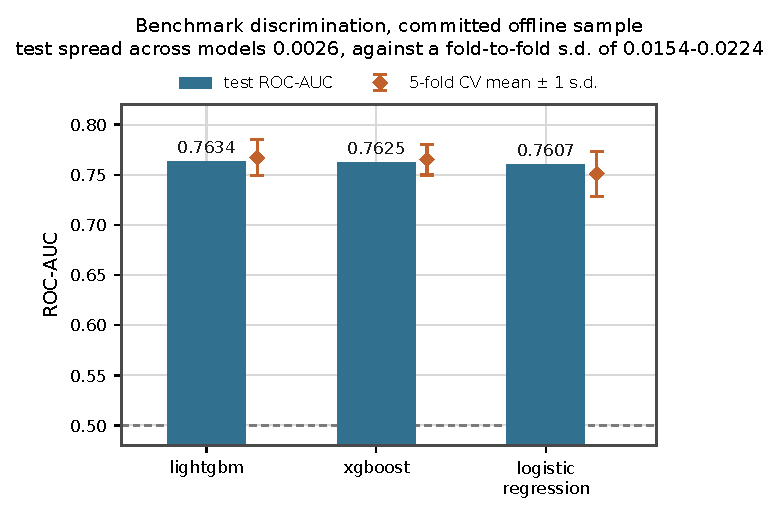
\includegraphics[width=0.60\textwidth]{fig_benchmark_roc_auc.pdf}
\caption{Test ROC-AUC per model with the cross-validation mean and standard
deviation alongside; the dashed line marks chance at $0.50$. The spread between
models is roughly an order of magnitude smaller than the fold-to-fold spread
within each model.}
\label{fig:bench}
\end{figure}

\section{Governance findings}

Table~\ref{tab:gates} gives the gate matrix. The overall verdict is FAIL for
every model, which is the intended outcome rather than a broken build: a
governance harness tuned so that everything passes is not measuring anything.

\begin{table}[htbp]
\centering
\small
\caption{Gate verdicts. The worst gate is the model's verdict.}
\label{tab:gates}
\begin{tabular}{llll}
\toprule
Gate & \code{lightgbm} & \code{xgboost} & \code{logistic\_regression} \\
\midrule
fairness           & FAIL & FAIL & FAIL \\
drift              & PASS & PASS & PASS \\
calibration        & WARN & WARN & WARN \\
uncertainty        & PASS & PASS & PASS \\
segment\_stability & FAIL & FAIL & WARN \\
\bottomrule
\end{tabular}
\end{table}

\subsection{Fairness: a gap on an attribute the model never saw}

The sharpest result is on \code{sex} under logistic regression. \code{sex} is
withheld from the feature matrix entirely, along with \code{marriage}, and kept
only as an audit column. The model nonetheless produces an equalized-odds
gap~\cite{hardt2016} --- here the larger of the max-min true-positive-rate spread
and the max-min false-positive-rate spread across groups --- of $\mathbf{0.1617}$,
past the $0.10$ fail limit, while passing demographic parity at $0.0459$.
Table~\ref{tab:sex} shows why: the gap is almost entirely in the true-positive
rate, where the false-positive-rate spread is only $0.0084$.

\begin{table}[htbp]
\centering
\small
\caption{Fairness detail for \code{sex}, logistic regression, decision threshold
$0.5$. Demographic parity gap $0.0459$ (pass); equalized-odds gap
$\mathbf{0.1617}$ (fail, limit $0.10$), $95\%$ interval $[0.050, 0.274]$.
$n_{\mathrm{def}}$ is the number of actual defaulters in the group, which is what
the TPR is estimated on.}
\label{tab:sex}
\begin{tabular}{lrrrrrr}
\toprule
\code{sex} & $n$ & $n_{\mathrm{def}}$ & Predicted default rate & Observed default rate & TPR & FPR \\
\midrule
male (1)   & 495 & 113 & 0.1333 & 0.2283 & \textbf{0.4071} & 0.0524 \\
female (2) & 755 & 163 & 0.0874 & 0.2159 & \textbf{0.2454} & 0.0439 \\
\bottomrule
\end{tabular}
\end{table}

That gap is a difference of two rates estimated on thin cells, and a report whose
argument is that raw rates from small cells need intervals owes its own headline
the same treatment. The TPR difference rests on 113 male and 163 female defaulters
in the test split. The Wald standard error for the difference of two independent
proportions is
%
\begin{equation}
\operatorname{s.e.}(\Delta\mathrm{TPR}) =
  \sqrt{\frac{\hat p_m(1-\hat p_m)}{n_m} + \frac{\hat p_f(1-\hat p_f)}{n_f}}
  = 0.0572,
\label{eq:tprse}
\end{equation}
%
giving a $95\%$ interval of $[0.050, 0.274]$ around the $0.1617$ point estimate. A
$20{,}000$-draw nonparametric bootstrap over the same rows, resampling within each
$(\text{sex}, \text{outcome})$ cell, agrees closely: standard error $0.0570$,
percentile interval $[0.050, 0.273]$. The point estimate therefore sits $1.08$
standard errors above the $0.10$ fail limit, and the interval comfortably contains
values below it.

Two readings follow, and both are worth keeping. The gate outcome is real: the
threshold is defined on the point estimate, the point estimate breaches it, and a
gate that waited for statistical significance before flagging a candidate
disparity would be the wrong instrument for the job --- the cost of a
false-positive FAIL is a review, the cost of a false-negative PASS is a deployed
model. But the evidence for a gap larger than $0.10$ \emph{specifically} is weak,
and the finding should not be quoted as though $0.1617$ were pinned down. What is
pinned down is the direction and the mechanism, not the magnitude.

The gap also depends on where the decision threshold is put, which matters here
because $0.5$ is a long way into the tail of a book with a $0.221$ base rate: only
$10.6\%$ of the test set is classified as a default at that threshold.
Table~\ref{tab:thresholds} recomputes the same gap at $0.30$ and at the
base-rate-matched $0.3153$, the threshold that classifies exactly as many
borrowers positive as actually default. The direction survives at every threshold;
the crossing of the $0.10$ limit does not. $0.5$ is the configured operating point
(\code{models.decision\_threshold}) and is where the gate runs, but a reviewer
reading Table~\ref{tab:sex} should know that the FAIL verdict is not robust to a
defensible alternative choice of threshold.

\begin{table}[htbp]
\centering
\small
\caption{Threshold sensitivity of the \code{sex} true-positive-rate gap, logistic
regression. Positive rate is the share of the test set classified as a default.
The base-rate-matched threshold is the $(1 - 0.2208)$ quantile of the predicted
probabilities. Standard errors are from Equation~\ref{eq:tprse}.}
\label{tab:thresholds}
\setlength{\tabcolsep}{5pt}
\begin{tabular}{lrrrrrl}
\toprule
Threshold & Positive rate & TPR male & TPR female & $\Delta$TPR & s.e. & Gate \\
\midrule
$0.30$                  & 0.2296 & 0.6018 & 0.5092 & 0.0926 & 0.0604 & WARN \\
$0.3153$ (base-rate)    & 0.2208 & 0.6018 & 0.5031 & 0.0987 & 0.0605 & WARN \\
$0.50$ (configured)     & 0.1056 & 0.4071 & 0.2454 & \textbf{0.1617} & 0.0572 & FAIL \\
\bottomrule
\end{tabular}
\end{table}

Two further things follow from Table~\ref{tab:sex} itself. First, a parity-only
fairness check would have signed this model off: predicted default rates are close
across the two groups, and it is recall on borrowers who actually defaulted that
is not --- a defaulting male applicant is identified $41\%$ of the time against
$25\%$ for a defaulting female applicant. Second, and more to the point, the model
produced that gap without ever reading the column, which is consistent with
correlated behavioural features carrying the signal back in.

That last clause is a hypothesis, so it is worth at least partially checking
rather than asserting. Training a model to recover \code{sex} from the same 49
retained predictors gives a test ROC-AUC of $0.588$ for logistic regression and
$0.607$ for LightGBM, against a $60.4\%$ female base rate. \code{Sex} is therefore
weakly but not negligibly recoverable from the features that survive exclusion:
enough for the repayment history to be a plausible route for the gap, not enough
to establish it as the route. Identifying the actual channel would need a feature
ablation this pipeline does not run, and the claim is left at that. What the
result does establish is the case that dropping a protected attribute does not
cover, and the reason the gate audits withheld attributes rather than treating
exclusion as sufficient. Logistic regression is also one of the two models that
reproduce bit-identically across platforms, so the figure is not an artefact of
the machine it was computed on.

The framework audits \code{age\_band} as well, and the contrast is instructive
rather than equivalent. \code{age} is used directly as a model feature --- 12th
of 49 by SHAP importance on LightGBM (Section~\ref{sec:shap}) --- and its
equalized-odds gap of $0.1600$ on LightGBM therefore reflects the model using an
input it was handed. That raises the question of whether the use is justified;
it is not evidence of a hidden proxy in the way the \code{sex} result is. The
60--80 band is excluded from the gate entirely: 10 test rows is below the
configured \code{min\_group\_size} of 50, and reporting a true-positive rate on
that is worse than reporting nothing.

\subsection{Calibration, drift and uncertainty}

Calibration warns on all three models. LightGBM's expected calibration
error~\cite{naeini2015} --- the bin-count-weighted mean absolute difference between
predicted probability and observed frequency over 15 equal-width reliability bins
--- is $0.0411$ against a warn limit of $0.03$, with maximum calibration error
$0.2266$ over the 14 bins that are populated and a mean predicted PD of $0.2060$
against an observed rate of $0.2208$: a slight systematic under-prediction of
$0.0148$. Drift passes cleanly, as it should on a random split: maximum feature PSI
is $0.0156$ across all 49 features, on \code{payment\_ratio\_mean}, with no feature
over the $0.10$ warn line. Uncertainty passes with $17.8\%$ of the test set above
the $0.60$-nat predictive-entropy threshold, against a warn line at $35\%$ and a
fail line at $55\%$ --- so the gate is not close to firing, and the figure is
reported because the share of the book the model refuses to call is worth knowing
even when it is acceptable. The bootstrap $95\%$ interval for LightGBM's ROC-AUC is
$[0.7022, 0.8097]$ --- a width of $0.107$, which is worth holding alongside the
$0.0026$ spread that separates the three models.

\subsection{Segment stability}

The stability gate fails LightGBM: 4 of 11 gated segments price outside their
credible interval, a ratio of $0.364$ against a fail limit of $0.30$. The
clearest breach is \code{graduate\_school | 30-40}, where the model's mean
predicted PD is $0.163$ against a shrunken posterior mean of $0.213$ with
interval $[0.187, 0.239]$, built from 560 reference borrowers. \code{university |
50-60} breaches in the same direction, $0.187$ against $[0.202, 0.276]$. Both
are under-predictions: the model prices default risk for these cells below their
noise-corrected historical experience. That is a provisioning concern, and no
aggregate metric in Table~\ref{tab:bench} surfaces it. Logistic regression warns
rather than fails here, at $0.273$.

\subsection{Robustness on the full 30{,}000 rows}
\label{sec:full}

Everything above is computed on the committed 5{,}000-row stratified sample, which
exists so that the pipeline, its tests and CI run without a network call. Rerunning
the identical configuration against the full 30{,}000-row dataset is the obvious
robustness check, and it changes what the headline can honestly be said to be.

Most of the picture holds or improves. The combined verdict is still FAIL for all
three models, and still on the fairness gate, for the same reason in kind: an
equalized-odds breach on a demographic attribute. Discrimination rises with the
extra data, to ROC-AUC $0.7781$ for both LightGBM and XGBoost and $0.7573$ for
logistic regression, on fold-to-fold standard deviations of $0.0069$--$0.0086$
rather than the $0.0154$--$0.0224$ of Table~\ref{tab:bench}. Calibration moves from
WARN to PASS on all three (ECE $0.0164$, $0.0156$, $0.0193$), which is what more
data should do to a calibration warning. Drift and uncertainty pass as before.
Segment stability passes for the tree models and warns for logistic regression, and
all 20 education $\times$ age-band cells are populated, so nothing is dropped.

The \code{sex} result does not survive at its sample magnitude. On the full data
the logistic-regression equalized-odds gap on \code{sex} falls to $0.0245$, with a
Wald $95\%$ interval of $[-0.021, 0.070]$ on 702 male and 957 female test-set
defaulters --- the same sign, roughly a sixth of the size, and a pass rather than a
fail. The two intervals overlap, so the estimates are not in formal contradiction;
$0.1617$ with a standard error of $0.0572$ is simply what an estimate near a
threshold does on 276 defaulters. What binds instead on the full data is
\code{age\_band}, at $0.1121$ to $0.1417$ across the three models: a failing gap on
the attribute the model is handed, not on the one withheld from it.

The reading that survives is that the mechanism is worth taking seriously and the
specific number is not. A withheld attribute can produce a measurable error-rate
gap; the gate finds it without being told to look for a proxy; and the same audit
run at six times the sample size still fails, on a different attribute. That the
\code{sex} effect is small enough on 30{,}000 rows to pass a $0.10$ limit is a more
useful finding than the sample figure was, and it is the argument this report makes
for shrinking segment rates, turned on its own headline. Regenerating
Tables~\ref{tab:bench}--\ref{tab:thresholds} against the full dataset, rather than
reporting it in prose here, is left as the next revision; the figures and the
worked examples throughout remain those of the offline sample.

\section{Cross-platform reproducibility}
\label{sec:repro}

On the same seed and the same sample hash, across Windows and Linux:

\begin{itemize}
\itemsep0.15em
\item \code{logistic\_regression} and \code{lightgbm} reproduce
      \textbf{bit-identically} --- every metric, every gate verdict, every
      credible interval.
\item The Bayesian layer reproduces bit-identically everywhere as well. That is an
      observation about these two platforms, not a guarantee: the layer runs no
      threaded reduction of its own, which removes the specific cause behind the
      XGBoost result below, but cross-platform bit-identity ultimately turns on the
      BLAS build and the floating-point behaviour underneath it. Being numpy/scipy
      only makes the outcome likely, not certain.
\item \code{xgboost} does \textbf{not}. Its histogram tree builder reduces
      floating-point sums in a thread- and platform-dependent order, so the same
      seed gives ROC-AUC $0.7672$ on Linux and $0.7625$ on Windows, with ECE
      $0.0320$ against $0.0438$.
\end{itemize}

That $0.0047$ spread is larger than the $0.0038$ margin between the top two
models on Linux, so \emph{which model wins depends on the machine it is run on}:
XGBoost on Linux, LightGBM on Windows. Table~\ref{tab:bench} reports the Windows
run for that reason, and the CI table in the repository README reports the Linux
run.

Every gate verdict in Table~\ref{tab:gates} is identical on both platforms,
which is the part worth keeping: the approval decision is stable even where the
leaderboard is not. A governance verdict that flipped with the host would be
useless, whereas a benchmark ranking that flips is merely unreliable. Anyone
needing a stable winner as well as a stable verdict should pin the platform or
set \code{models.enabled} to a single model.

\section{Explainability}
\label{sec:shap}

SHAP runs on whichever model the selection metric picks, which on this run is
LightGBM. Explainer choice is by model family --- exact tree SHAP for the
boosters, exact linear SHAP for the scaled logistic pipeline --- so neither path
uses sampling approximation~\cite{lundberg2017}. Both output on the log-odds
scale, where contributions are additive: $\sigma(\text{base} + \sum
\text{SHAP})$ recovers the predicted probability exactly. A mean absolute SHAP
value is therefore movement in log-odds, not a change in probability of default.

\begin{figure}[htbp]
\centering
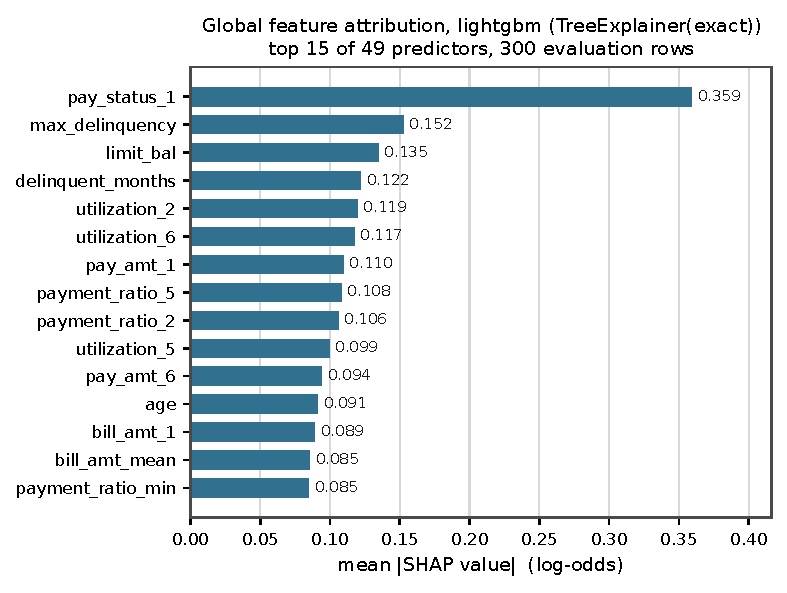
\includegraphics[width=0.64\textwidth]{fig_shap_importance.pdf}
\caption{Global feature attribution for LightGBM, exact \code{TreeExplainer},
top 15 of 49 predictors over 300 evaluation rows against 100 background rows.}
\label{fig:shap}
\end{figure}

Figure~\ref{fig:shap} shows the result. Most recent repayment status
(\code{pay\_status\_1}, $0.359$) dominates at more than twice the next feature,
followed by \code{max\_delinquency} ($0.152$), \code{limit\_bal} ($0.135$) and
\code{delinquent\_months} ($0.122$). Delinquency history and credit limit
carrying the model is consistent with the source paper~\cite{yeh2009}. The
pipeline also writes per-feature contribution breakdowns for three individual
borrowers --- the highest-risk, the lowest-risk, and the most uncertain in the
sample --- as JSON, in the form an adverse-action review needs.

\section{Dataset, tech stack, and reproducing this report}

The data is UCI Machine Learning Repository dataset 350, \emph{Default of Credit
Card Clients}~\cite{yeh2009,uci350}: 30{,}000 Taiwanese credit-card customers,
23 features covering six months of billing and repayment history plus limited
demographics, and a binary target for default on the next payment, at a base
default rate of $22.1\%$. It is distributed under CC BY 4.0; the repository
commits a 5{,}000-row class-stratified draw (base rate $22.12\%$) under the same
licence, so the pipeline, its tests, and the CI smoke job run with no network
call.

Models are scikit-learn \code{LogisticRegression}, \code{xgboost} and
\code{lightgbm}; the Bayesian layer is numpy and scipy only; configuration is
pydantic v2 with \code{extra="forbid"}; explainability is \code{shap}; tracking
is MLflow with a local JSON fallback. CI runs ruff, pytest on Python 3.12 and
3.13, and an end-to-end smoke job that asserts both scorecards and all three
model cards were written, that three models were benchmarked with five gates
each, that every ROC-AUC beat chance, and that the shrinkage prior was fitted.

Everything in this report regenerates from the tagged release:

\begin{quote}
\code{git clone https://github.com/asynced24/bayesian-credit-risk-gate.git}\\
\code{cd bayesian-credit-risk-gate \&\& git checkout v1.0.0}\\
\code{pip install -r requirements.txt}\\
\code{python main.py --sample}\\
\code{python docs/figures/generate\_figures.py}\\
\code{python main.py}\ \ \ \ (full 30{,}000 rows, Section~\ref{sec:full}; needs network once)
\end{quote}

Tables~\ref{tab:bench}--\ref{tab:thresholds} are taken from the scorecard JSON that
the \code{--sample} run writes into \code{reports/}. The four figures come from
\code{generate\_figures.py}, and Figure~\ref{fig:eb} re-fits the shrinkage model
directly rather than reading a cached artefact. The final command fetches and
caches the full dataset and produces
the run reported in Section~\ref{sec:full}; every subsequent invocation reads the
cache. Python 3.12 or newer is required, since the pinned numpy, scipy, xgboost and
shap releases all declare \code{Requires-Python >= 3.12}.

\begin{thebibliography}{9}
\footnotesize
\setlength{\itemsep}{2pt}

\bibitem{yeh2009}
Yeh, I.-C., \& Lien, C.-H. (2009).
The comparisons of data mining techniques for the predictive accuracy of
probability of default of credit card clients.
\emph{Expert Systems with Applications}, 36(2), 2473--2480.

\bibitem{uci350}
UCI Machine Learning Repository, dataset 350: \emph{Default of Credit Card
Clients}. Distributed under CC BY 4.0.
\url{https://archive.ics.uci.edu/dataset/350/default+of+credit+card+clients}

\bibitem{gelman2013}
Gelman, A., Carlin, J. B., Stern, H. S., Dunson, D. B., Vehtari, A., \&
Rubin, D. B. (2013). \emph{Bayesian Data Analysis}, 3rd edition. CRC Press.

\bibitem{hardt2016}
Hardt, M., Price, E., \& Srebro, N. (2016). Equality of opportunity in
supervised learning. \emph{Advances in Neural Information Processing Systems},
29.

\bibitem{lundberg2017}
Lundberg, S. M., \& Lee, S.-I. (2017). A unified approach to interpreting model
predictions. \emph{Advances in Neural Information Processing Systems}, 30.

\bibitem{naeini2015}
Naeini, M. P., Cooper, G. F., \& Hauskrecht, M. (2015). Obtaining well
calibrated probabilities using Bayesian binning. \emph{Proceedings of the AAAI
Conference on Artificial Intelligence}, 29.

\end{thebibliography}

\end{document}
